\documentclass[12pt, a4paper, openany]{report} %, BCOR0mm scrbook

% scrartcl ist eine abgeleitete Artikel-Klasse im Koma-Skript
% bibliography=totoc: Literaturverzeichnis im Inhaltsverzeichnis
% zur Kontrolle des Umbruchs Klassenoption draft verwenden
%BCOR: Bindekorrektur


% die folgenden Packete erlauben den Gebrauch von Umlauten und ß
% in der Latex Datei
\usepackage[utf8]{inputenc}
% \usepackage[latin1]{inputenc} %  Alternativ unter Windows
\usepackage[T1]{fontenc}
%\usepackage[ngerman]{babel}


\usepackage[paper=a4paper,left=25mm,right=25mm,top=25mm,bottom=25mm]{geometry}
\usepackage[pdftex]{graphicx}
\usepackage{subfigure}
\usepackage{latexsym}
\usepackage{amsmath,amssymb,amsthm}
\usepackage[export]{adjustbox}
\usepackage{pdfpages}
% deutsches Literaturverzeichnis
\usepackage[numbers,round]{natbib}

%neue Seite für jedes Kapitel
%\usepackage{titlesec}
%\newcommand{\sectionbreak}{\clearpage}

% Umgebungen für Definitionen, Sätze, usw.
% Es werden Sätze, Definitionen etc innerhalb eines Chapters mit
% 1.1, 1.2 etc durchnummeriert, ebenso die Gleichungen mit (1.1), (1.2) ..
\newtheorem{Satz}{Satz}[chapter]
\newtheorem{Lemma}[Satz]{Lemma}
\newtheorem{Korollar}[Satz]{Korollar}

\theoremstyle{definition}	
\newtheorem{Definition}[Satz]{Definition}
\newtheorem{Beispiel}[Satz]{Beispiel}
\newtheorem{Bemerkung}[Satz]{Bemerkung}
                    
\numberwithin{equation}{chapter} 

% einige Abkuerzungen
\newcommand{\C}{\mathbb{C}} % komplexe
\newcommand{\K}{\mathbb{K}} % komplexe
\newcommand{\R}{\mathbb{R}} % reelle
\newcommand{\Q}{\mathbb{Q}} % rationale
\newcommand{\Z}{\mathbb{Z}} % ganze
\newcommand{\N}{\mathbb{N}} % natuerliche
\DeclareMathOperator{\sign}{sign}



\begin{document}

  % Keine Seitenzahlen im Vorspann
  \pagestyle{empty}
\noindent
\begin{titlepage}
	
	\newcommand{\HRule}{\rule{\linewidth}{0.5mm}} % Defines a new command for the horizontal lines, change thickness here
	
	\center % Center everything on the page
	
	%----------------------------------------------------------------------------------------
	%	HEADING SECTIONS
	%----------------------------------------------------------------------------------------
	\hspace*{5.0cm}\\[4cm]

	\textsc{\LARGE Mathematical Aspects\\[0.2cm] of Machine Learning}\\[0.5cm] % Major heading such as course name
	\textsc{\large Report}\\[2cm] % Minor heading such as course title
	
	%----------------------------------------------------------------------------------------
	%	TITLE SECTION
	%----------------------------------------------------------------------------------------
	
	\HRule \\[0.8cm]
	{ \huge \bfseries Digit Recognition\\ with Support Vector Machine}\\[0.8cm] % Title of your document
	\HRule \\[1.5cm]
	
	%----------------------------------------------------------------------------------------
	%	AUTHOR SECTION
	%----------------------------------------------------------------------------------------
	
	\begin{minipage}{0.4\textwidth}
		\begin{flushleft} \large
			\emph{Authors:}\\
			Lisa \textsc{Gaedke-Merzhäuser} \\% Your name
			Paul \textsc{Korsmeier}\\
			Lisa \textsc{Mattrisch}\\
			Vanessa \textsc{Schreck}\\
		\end{flushleft}
	\end{minipage}
	~
	\begin{minipage}{0.4\textwidth}
		\begin{flushright} \large
			\emph{} \\
			 \textsc{} % Supervisor's Name
		\end{flushright}
	\end{minipage}\\[2cm]

	
	
\end{titlepage}

\cleardoublepage
  % Ab sofort Seitenzahlen unten mittig
  \pagestyle{plain}

\chapter*{Problem Statement}
Our main goal is to correctly identify handwritten digits based on the MNIST  ("Modified National Institute of Standards and Technology") data set.
This data set consists of 42,000 gray-scale images. Each image is 28 pixels in height and 28 pixels in width. Each pixel has a single pixel-value associated with it, indicating the lightness or darkness of that pixel \cite{kaggel}.

\begin{figure}[h]
	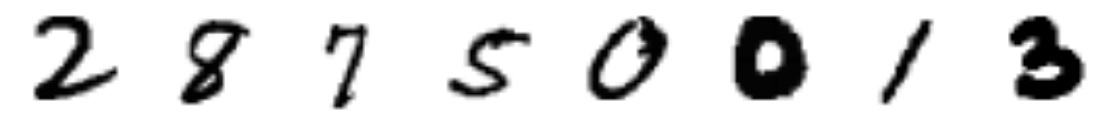
\includegraphics[width=1\textwidth, center]{Digits2}
	\caption{Visualization of eight of these images}
\end{figure}


Formally speaking, we have points  $\{x_i\}_{i=1}^l \subset \R^{28^2}$ with respective labels from $\{0,1,\ldots, 9\}$. Our goal is now to find a classification function $f$ that gives for each of these points a prediction $f(x) \in \{0,1,\ldots, 9\}$ which ideally matches the actual label.\\

There are several ways to achieve this goal, one of which are the concept of {kernelized} support vector machines (SVM). The main idea behind this algorithm is to not only separate the data according to their labels, but also do so in a way that is as reasonable as possible, i.e. we want to maximize the distance of the data to the decision boundary. We first transfer the data with a feature map $\Phi$ into a suitable feature space and look for a linear separation there.\\

From this notion, one particular problem arises: The SVM is a binary classifier, i.e. it can only handle data that is divided into two classes. We therefore decided to compare different ways to deal with this obstacle, generalizing the application of SVMs to multiclass  classification problems (cf. Section \ref{ch_multiclass}). The methods that we considered all combine several instances of the SVM in its original form, classifying according to labels $\{\pm 1\}$.\\

We can summarize this binary classification problem in the objective of finding a decision function of the form
\begin{equation*}
f(x) = \sign \left(w^T\Phi(x) + b\right).
\end{equation*}


\subsection{Binary Support Vector Machine}


Approaching binary support vector machines from a more technical side, we find that they aim to find the maximum margin hyperplane in the feature space, i.e. the goal is to maximize the margin while softly penalizing points that lie on the wrong side of the boundary or inside the margin \cite{Bishop2006}. Dualizing this optimization problem, we obtain the following equivalent quadratic program:

\begin{eqnarray}
	\text{minimize} & d(\alpha) := \frac{1}{2} \alpha^T Q \alpha - 1^T \alpha \label{eq:dual_problem} \\ 
	\text{s.t.} &  0 \leq \alpha \leq C  \quad \text{and} \quad 	y^T \alpha = 0,	\nonumber
\end{eqnarray}

where $\alpha$ is the dual variable, $Q_{ij} = y_i y_j k(x_i,x_j)$, $k$ the kernel function and $C = 1/(2 \lambda l)$ for the penalty term $\lambda$ of the soft margin SVM.
After finding the optimal solution $\alpha^*$ of this program, we can formulate the resulting decision function as
\begin{equation*}
f(x) = \operatorname{sgn}\left(\sum_{i=1}^{l}\alpha^*_i y_i k(x_i,x_j)+b\right).
\end{equation*}
Note that only data points $x_i$ with $\alpha_i \neq 0$ appear in the decision function. Those points are called \textit{support vectors}.\\
By analysing primal, dual and the corresponding KKT conditions, we find that any $x_i$ with $\alpha_i = C$ was correctly classified and lies exactly on the margin boundary, and any $x_i$ with $0<\alpha_i < C$ lies either inside the margin or on the wrong side of the margin. Additionally, any data points $x_i$ on the (correct) margin boundary must satisfy $y_i f(x_i) = 1$. We can use this property to find the parameter $b$ \cite{Bishop2006}. Hence, if we succeed to find an optimal solution to \eqref{eq:dual_problem}, we have everything we need to construct the decision function.





\chapter*{Support Vector Machine}


The Support Vector Machine (SVM) is a binary classifier that aims to find the maximum margin hyperplane in the feature space, i.e. the goal is to maximize the margin while softly penalizing points that lie on the wrong side of the boundary or inside the margin \cite{Bishop2006}. Dualizing this optimization problem, we obtain the following equivalent quadratic program:
\begin{equation*}
\begin{aligned}
& \underset{0 \leq \alpha \leq C}{\text{maximize}}
& & \sum_{i = 1}^{l}\alpha_i - \frac{1}{2} \sum_{i, j = 1}^{l}\alpha_i  \alpha_j y_i y_j k(x_i, x_j)
\end{aligned}
\end{equation*}
where $\alpha$ is the dual variable, $q_{ij} = y_i y_j k(x_i,x_j)$, $k$ the kernel function and $C = 1/2 \lambda l$ for the penalty term $\lambda$ of the soft margin SVM.
After finding the optimal solution $\alpha^*$ of this program, we can formulate the resulting decision function as
\begin{equation*}
f(x) = \operatorname{sgn}\left(\sum_{i=1}^{l}\alpha^*_i y_i k(x_i,x_j)+b\right).
\end{equation*}
Note that only data points $x_i$ with $\alpha_i \neq 0$ appear in the decision function. Those points are called \textit{support vectors}. By analysing primal, dual and the corresponding KKT conditions, we find that any $x_i$ with $\alpha_i = C$ was correctly classified and lies exactly on the margin boundary, and any $x_i$ with $0<\alpha_i < C$ lies either inside the margin or on the wrong side of the margin. Additionally, any data points $x_i$ on the (correct) margin boundary must satisfy $y_i\cdot f(x_i) = 1$. We can use this property to find the parameter $b$ \cite{Bishop2006}.



\chapter*{Solving the optimization problem with SMO}
Let $\alpha$ be some feasible variable for Problem (\ref{dual_problem}). Defining
\begin{equation}
F_i(\alpha) := y_i (\partial_i d)(\alpha) = \sum_{i = 1}^l \alpha_j y_j k(x_i,x_j) - y_i \quad \text{for} \quad i = 1,\ldots,l,
\end{equation}
by careful computation we find that the KKT optimality conditions for a solution of Problem (\ref{dual_problem}) (which are both necessary and sufficient, since Q is spsd), are equivalent to the -- much simpler looking -- pairwise condition
\begin{equation}\label{equiv_KKT}
b_{up}(\alpha) := \min_{i \in I_{up}(\alpha)} F_i(\alpha) \geq \max_{j \in I_{low}(\alpha)} F_j(\alpha) =: b_{low}(\alpha),
\end{equation}
where $I_{up}(\alpha)$ and $I_{low}(\alpha)$ are subsets of the index set $\{1,\ldots,l\}$ defined by
\begin{align}
I_{up}(\alpha) &:= \{ i  \mid  \alpha_i < C \text{ and } y_i = 1 \text{ or } \alpha_i > 0 \text{ and } y_i = -1 \} \\
I_{low}(\alpha) &:= \{ j \mid \alpha_j < C \text{ and } y_j = -1 \text{ or } \alpha_j > 0 \text{ and } y_j = 1 \}.
\end{align} 
Any pair $(i,j) \in I_{up}(\alpha) \times I_{low}(\alpha)$ with $F_i(\alpha) < F_j(\alpha)$ is thus called a \textit{violating pair} and an objective equivalent to solving Problem (\ref{dual_problem}) is to change $\alpha$ so as to remove all such violating pairs. Since a priori we do not know if the solution $\alpha^*$ fulfils (\ref{equiv_KKT}) strictly or not, we define, for some small tolerance $\tau > 0$, a $\tau$-violating pair as some $(i,j) \in I_{up}(\alpha) \times I_{low}(\alpha)$ which satisfies $F_i(\alpha) < F_j(\alpha) - \tau$ and require that all $\tau$-violating pairs be removed, or equivalently, 
\begin{equation}\label{tau_KKT}
b_{up}(\alpha) \geq b_{low}(\alpha) - \tau.
\end{equation}
It holds that any algorithm of the following form terminates after finitely many steps:
\begin{algorithm}[General SMO type algorithm] Let $\tau > 0$. Initialize $k = 0 $ and $\alpha = 0$ and generate iterates $\alpha^k$, $k \in \mathbb{N},$ as follows: 
\begin{enumerate}
\item If $\alpha^k$ satisfies (\ref{tau_KKT}), stop. Else choose a $\tau$-violating pair $(i,j) \in I_{up}(\alpha^k) \times I_{low}(\alpha^k)$.
\item Minimize $d$ varying only $\alpha^k_i$ and $\alpha^k_j$, leaving $\alpha^k_n$ fixed for $n \notin \{i,j\}$ and respecting the constraints of Problem (\ref{dual_problem}) to obtain $\alpha^{\text{new}}$.
\item Set $k := k+1$, $\alpha^k := \alpha^{\text{new}}$ and go to Step 1.
\end{enumerate}
\end{algorithm}


\chapter{Multi Class Classification Problem}
Support Vector Machines are binary classifiers, meaning that there only two possible output labels. Usually, one chooses them to be $1$ and $-1$. Our problem, however, was to classify unknown data into one out of ten different categories. Since rewriting the SVM algorithm to produce a separation into multiple classes is linked to great effort, we opt for finding a way to combine several SVMs, which together would be able to choose from more than one label. There are a number of well known strategies tackling this issue. Let us first look at two very intuitive but also primitive strategies. The first one is known as One-vs-All classification. In this approach one trains as many SVMs as there are classes, i.e. ten in our case, and sets labels so that the $i$-th SVM has all training data with label $i$ set to 1 and everything else to $-1$. 

....

This approach has many issues. Not uniquely classified. Advantage low compute time, one has to at least expect to train $10$ binary classifiers to divide into $10$ different categories. depends on which one first...? some areas several labels...  

The other possibility is called One-vs-One classification. Here one only ever considers the data corresponding to two classes and sets one label to $1$ and the other one to $-1$. ... 
In our case this would mean training $45$ SVMs (the number arises from the binary coefficient of 10 choose 2...). advantage/disadvantage

We only tried the first approach since as just mentioned the compute time for the second one was simply too high for us considering that we have a very large amount of training data. In the One-vs-All results were very very disappointing. In the case of a linear as well as a Gaussian kernel ... In the linear case this can be explained by the fact that our training data was simply not linearly seperable. 
Hence we added in an additional feature. We computed the barycenters of the data points of each class. When a data point could not be uniquely classified we would give it the label of the barycenter it was closest to. This method led to a major improvement of our results. Our algorithm now labeled about 60\% of our data correctly (... see appendix).  Nevertheless the result was still not satisfactory. 

So we decided to focus our attention on a different approach: Error Correcting Output Codes. 
\\
subheading? \\
\\
They are easiest to explain considering a concrete example. We trained 15 different classifiers $f_i$. 

\begin{table}[ht!]
	\centering
	\caption{Error Correcting Output Codes}
	\label{Codewords}
	\begin{tabular}{|l|l|l|l|l|l|l|l|l|l|l|l|l|l|l|l|}
	\hline
	Class	& $f_0$ & $f_1$ & $f_2$ & $f_3$ & $f_4$ & $f_5$ & $f_6$ & $f_7$ & $f_8$ & $f_9$ & $f_{10}$ & $f_{11}$ & $f_{12}$ & $f_{13}$ & $f_{14}$ \\ \hline \hline
	0	& 1 & 1 & -1 & -1 & -1 & -1 & 1 & -1 & 1 & -1 & -1 & 1 & 1 & -1 & 1 \\ \hline
	1	&  &  &  &  &  &  &  &  &  &  &  &  &  &  & \\ \hline
	2	&  &  &  &  &  &  &  &  &  &  &  &  &  &  & \\ \hline
	3	&  &  &  &  &  &  &  &  &  &  &  &  &  &  & \\ \hline
	4	&  &  &  &  &  &  &  &  &  &  &  &  &  &  & \\ \hline
	5	&  &  &  &  &  &  &  &  &  &  &  &  &  &  & \\ \hline
	6	&  &  &  &  &  &  &  &  &  &  &  &  &  &  & \\ \hline
	7	&  &  &  &  &  &  &  &  &  &  &  &  &  &  & \\ \hline
	8	&  &  &  &  &  &  &  &  &  &  &  &  &  &  & \\ \hline
	9	&  &  &  &  &  &  &  &  &  &  &  &  &  &  & \\ \hline
	\end{tabular}
\end{table}  

The rows of the table show what class is assigned what label depending on each classifier. For example $f_0$ assigns $1$'s to all even numbers and $-1$'s to all odd numbers. This way each class has a string of $1$'s and $-1$'s it corresponds to which is also called its codeword. The codewords are chosen such that their Hamming distance (i.e. the number of entries where they differ) is maximized. In our case each codeword has a Hamming distance of at least six to any of the others strings. Now when one wants to label an unknown data point each of the classifiers assigns it a label and one gets an output string of 15 digits. We classify the data point according the codeword it has the least Hamming distance to. The name error correcting output codes is derived from the fact that we can for example three classifiers can misclassify a data point and we will still get the correct result. Depending on the difficulty of the problem one could choose more or less classifiers and hece in-or decrease the Hamming distance of the set of codewords. We took these codewords from ... and yielded much better results than with the approaches mentioned above. Our precise implementation can be found on page... in the appendix. 

When choosing ... many training points and .... many testing points our algorithm was correct in ... of the cases. Include things here...?

Linear and Gaussian.

In general ECOC?

Where do we bring in cross validation?

%Es wurden auch einige Eigenschaften der Fatou-Menge beleuchtet, unser Hauptaugenmerk lag jedoch auf der Julia-Menge.Trotzdem die Iterierten auf der Fatou-Menge normal sind und die Dynamik der Funktion hier in dem Sinne gut zu beschreiben ist, dass benachbarte Punkte unter Iteration ein ähnliches Verhalten zeigen, hat sie doch viele interessante Eigenschaften. Beispielsweise kann man die Zusammenhangskomponenten der Fatou-Menge klassifizieren und wird feststellen, dass es recht wenige Typen gibt. Mehr dazu findet sich in \cite{Schleicher}.


\chapter{Results \& Conclusions}
This is the largest programming project any one of has ever worked on and neither of us had done much with Python before or had any other machine learning experience. So at any given time there was always a great variety of difficulties at hand. And because we implemented everything ourselves the problem could be literally anywhere, from misunderstanding the pseudocode we used, over float and integer division or git merging issues to immense troubles with the internal solvers for the optimization problem. But because of that every little success was a source of joy which grew with every working block of code we managed to compile.

\smallskip
The overall structure of our program looks as follows. We wrote our own \texttt{mySVMclass}, which is a self contained object with a number of attributes and callable functions, which includes the \texttt{SMOsolver} and \texttt{crossValidation}. We then have separate .ipynb notebooks for the two classification algorithms where we specify training data sets, the kernel, the different parameters and create instances of our \texttt{mySVMclass}. Especially in the case of the gaussian kernel finding suitable parameters was very essential. We therefore wrote a separate notebook where we systematically test them and determine which ones seem optimal. We also automatically save our trained SVMs for the different sized training data in binary format. We also visualized toy data sets in lower dimensions to better understand how our algorithms behave in different cases.

\begin{table}[ht!]
	\centering
	\caption{\textbf{Overview Results of Correctly Classified Digits}}
	\begin{tabular}{|l|l|l|l|l|l|l|l|l|l|l|l|} \hline
		\multicolumn{1}{|p{1.8cm}|}{\vspace*{.7 cm}\# training points} &
		\multicolumn{1}{p{1.8cm}|}{\vspace*{0 cm}\hbox{One-vs-All} uniquely classfied, linear} &
		\multicolumn{1}{p{1.8cm}|}{\vspace*{0 cm}\hbox{One-vs-All} with bary- centers, linear} &
		\multicolumn{1}{p{1.8cm}|}{\vspace*{0 cm}\hbox{One-vs-All} uniquely classfied, Gaussian} &
		\multicolumn{1}{p{1.8cm}|}{\vspace*{0 cm}\hbox{One-vs-All} with bary-centers, Gaussian} &
		\multicolumn{1}{p{1.8cm}|}{\vspace*{.7 cm}ECOC, \hbox{linear}} &
		\multicolumn{1}{p{1.8cm}|}{\vspace*{.7 cm}ECOC, Gaussian} \\ \hline \hline
		500	& 65.9\% & 74.1\% & 75.4\% & 83.3\% & 74.2\% & 87.4\% \\ \hline
		1000	& 68.2\% & 75.0\% & 84.3\% & 89.0\% & 78.0\% & 92.7\% \\ \hline
		2000	& 70.2\% & 76.4\% & 89.8\% & 91.9\% & 77.8\% & 94.3\% \\ \hline
		5000	& 70.0\% & 73.8\% & 88.9\% & 91.6\% & 82.0\% & 95.2\% \\ \hline
		10000	& 64.6\% & 67.5\% & 88.0\% & 90.6\% & 82.5\% & 95.4\% \\ \hline
	\end{tabular}
\end{table}

\smallskip
Our given data set included 42,000 handwritten digits. We never used all of them for training because this large amount of training data simply exceeded our available compute power. But from the table below we can see that it would probably not have improved our results considerably or might even have worsened them. And this way we always had engouh labeled data to test and verify our results with. In the table you can find the results of the different multi-class classifiers. For the One-vs-All approach we give numbers for how many labels were found correctly with and without using additional classification by location of the barycenters, so that one can really see how many uniquely classified data points are labeled correctly. The percentages are derived from always testing with 1,000 data points that were of course not used for training beforehand. Unsurprisingly ECOC had longer run times than the One-vs-All classifier, it has to train $15$ instead of only $10$ and the computation with the Gaussian kernel took longer than with the linear kernel, which was also to be expected because of its higher complexity (more detail?). For 10,000 training points ECOC with linear kernel took $1$h $16$ min and ECOC with gaussian kernel took $2$ h $26$ min for training.  

\smallskip
As expected from theoretical considerations the Error-Correcting Output Codes performed better than the One-vs-All classification for training sets of any size. However we were surprised how well One-vs-All with the gaussian kernel worked in the end. Every picture of a hand-written digit gets turned into a vector of size $784$  ($=28^2$), it was not clear that the output data would be anywhere close to being linearly separable so we were also suprised to see the linear classifiers working at all, especially in the first case were not a single ambiguity or mistake could be corrected. With an increase of training points the results first increase across the board. The performance of classifiers with linear kernel then often starts to decrease, sometimes drastically, with training sets of size 2,000. We assume that this phenomenon occurs because the more training data we have the harder it gets to linearly separate it. 

% Ich hätte ganz links oben gerne eine schräge Linie
% \lft{n}\rt{k}}
% \lft{classifier}\rt{no of training points}	


We have learned a lot in the past 4 weeks and although this program does not (yet?) win us a kaggle competition we are in general (very) satisfied with the overall outcome of the project and especially with our success rate of over $95$\%.


\bibliography{Report_bib}
  \bibliographystyle{alphadin}

%\cleardoublepage
%\includepdf{Selbstaendigkeitserklaerung.pdf}  



\end{document}

